\documentclass[11pt,letterpaper]{article}
\usepackage[utf8]{inputenc}
\usepackage[T1]{fontenc}
\usepackage[spanish]{babel}
\usepackage[margin=2.3cm]{geometry}
\usepackage{newtxtext,newtxmath}
\usepackage{amsmath}
\usepackage{booktabs}
\usepackage{graphicx}
\usepackage{float}
\usepackage{enumitem}
\usepackage{xcolor}
\usepackage{hyperref}
\hypersetup{colorlinks=true,urlcolor=blue!60!black,linkcolor=black}
\setlist{nosep,leftmargin=1.4em}
\setlength{\parskip}{0.5em}
\setlength{\parindent}{0pt}
\newcommand{\g}[1]{\texttt{#1}}

\begin{document}

\begin{center}
{\Large\bfseries Proyecto No. 2: Simplificación de gramáticas y algoritmo CYK}\\[0.4em]
Teoría de la Computación — Universidad del Valle de Guatemala\\[0.3em]
Samuel Robledo — 241282 \qquad 19 de octubre de 2026\\[0.2em]
\url{https://github.com/samuelrobledo52/Proyecto2-TC}
\end{center}

\section{Diseño}

El programa lee una gramática desde un archivo, la convierte a CNF y valida frases con CYK. Está dividido en cinco módulos:

\begin{itemize}
\item \g{gramatica.py}: guarda las producciones como \g{variable → lista de tuplas}; la tupla vacía es $\varepsilon$. Lo que nunca aparece como cabeza es terminal.
\item \g{cnf.py}: una función por paso de simplificación.
\item \g{cyk.py}: llena la tabla y separa la frase en tokens, aunque venga sin espacios.
\item \g{arbol.py}: arma el parse tree desde la tabla y lo dibuja con Graphviz.
\item \g{main.py}: recibe la gramática y las frases y guarda todo en \g{resultados.txt}.
\end{itemize}

\section{Conversión a CNF}

Se sigue el orden de Hopcroft, porque cada paso puede dejar casos que el siguiente limpia:

\begin{enumerate}
\item Si el inicial es anulable y aparece en un cuerpo, se agrega $S_0\to S$.
\item Se eliminan las producciones $\varepsilon$ generando las combinaciones sin anulables.
\item Se eliminan las unitarias con los pares $(A,B)$ tales que $A\Rightarrow^* B$.
\item Se quitan los símbolos que no generan y luego los que no son alcanzables.
\item Los terminales en cuerpos de largo 2 o más se cambian por variables ($L\to($, $R\to)$, $P\to+$, $M\to*$).
\item Los cuerpos largos se parten en pares con variables nuevas $C_1, C_2, \dots$
\end{enumerate}

Con \g{1.txt} se obtiene la misma gramática de \g{1-cnf.txt}; solo cambian los nombres ($Z,W,V$ pasan a ser $C_1,C_2,C_3$):
\[
\begin{aligned}
E &\to TX \mid FY \mid LC_1 \mid id & X &\to PC_2 \mid PT & T &\to FY \mid LC_1 \mid id\\
Y &\to MC_3 \mid MF & F &\to LC_1 \mid id & C_1 &\to ER,\ C_2\to TX,\ C_3\to FY
\end{aligned}
\]
La gramática del enunciado ya está en CNF, así que ningún paso la cambia.

\section{Algoritmo CYK}

$T[i][j]$ contiene las variables que generan $w_i\cdots w_j$. Cada celda se calcula con celdas de subcadenas más cortas:
\[
T[i][i]=\{A \mid A\to w_i\},\qquad
T[i][j]=\{A \mid A\to BC,\ B\in T[i][k],\ C\in T[k+1][j],\ i\le k<j\}
\]
La frase se acepta si $S\in T[1][n]$, con costo $O(n^3|G|)$. Para el árbol, cada celda guarda también de dónde salió cada variable ($k$, $B$, $C$). El tiempo se mide solo sobre el llenado de la tabla.

\section{Ejemplos y pruebas}

\begin{center}\small
\begin{tabular}{@{}lcr@{\qquad}lcr@{}}
\toprule
Frase & Res. & ms & Expresión & Res. & ms\\ \midrule
She eats a cake with a fork & SÍ & 0.032 & \g{(id*id)+id} & SÍ & 0.035\\
The cat drinks the beer & SÍ & 0.035 & \g{id+id*id} & SÍ & 0.027\\
she cuts the meat with a knife in the oven & SÍ & 0.085 & \g{id*(id+id)*id} & SÍ & 0.047\\
he cooks & SÍ & 0.013 & \g{((id))} & SÍ & 0.030\\
she eats cake & NO & 0.007 & \g{id+} & NO & 0.010\\
the dog eats with a fork the soup & NO & 0.026 & \g{(id*id} & NO & 0.011\\
she eats a pizza & NO & 0.008 & \g{()} & NO & 0.003\\
\bottomrule
\end{tabular}
\end{center}

\emph{She eats cake} falla porque $NP$ necesita determinante, \emph{the dog eats with a fork the soup} porque no existe $VP\to VP\ NP$ y \emph{pizza} no es terminal.

\begin{figure}[H]
\centering
\begin{minipage}{0.55\textwidth}\centering
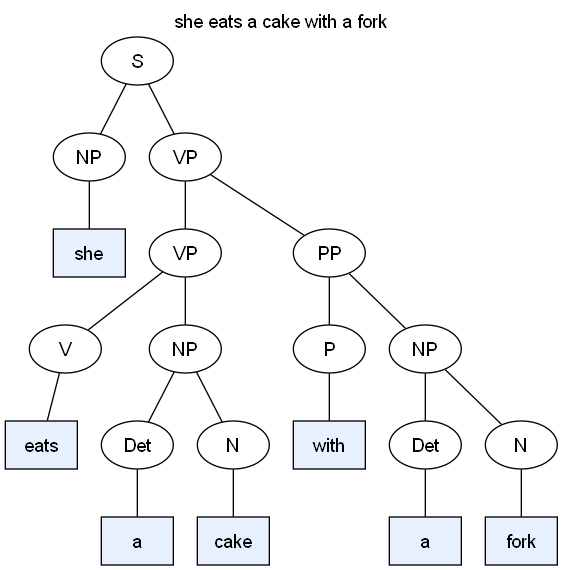
\includegraphics[width=0.85\linewidth]{arbol_ingles.png}
\end{minipage}\hfill
\begin{minipage}{0.4\textwidth}\centering
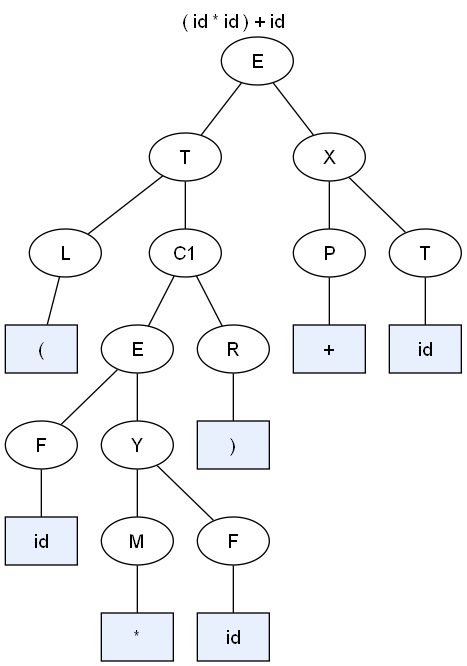
\includegraphics[width=0.7\linewidth]{arbol_expr.png}
\end{minipage}
\end{figure}

Para revisar la conversión, \g{pruebas/equivalencia.py} compara la gramática original (con un parser de Earley) contra CYK sobre la CNF. Se probaron 3\,000 gramáticas aleatorias y todas las cadenas cortas de \g{1.txt} y del enunciado, sin diferencias.

\section{Discusión}

\textbf{Obstáculos.} El orden de los pasos importaba: si se quitaban las unitarias antes que $\varepsilon$, volvían a aparecer. En \g{1.txt} ya existe $T$, así que los nombres nuevos se validan para no chocar. Agregar siempre $S_0$ duplicaba las producciones de $E$, por eso solo se agrega cuando hace falta. Las expresiones vienen sin espacios y las frases con mayúsculas o punto, y eso se resolvió en la tokenización. Los tiempos son muy pequeños y cambian entre corridas.

\textbf{Recomendaciones.} Guardar todas las derivaciones por celda permitiría ver todos los árboles de una frase ambigua. La gramática del enunciado no tiene $NP\to NP\ PP$, por lo que \emph{the cat with a fork eats} se rechaza. Con muchos anulables en un mismo cuerpo, la CNF crece bastante.

\vfill
\noindent\rule{0.35\textwidth}{0.4pt}\\
{\footnotesize Se utilizó Claude como apoyo en la implementación y la documentación. Todo el contenido fue revisado, probado y validado por mí.}

\end{document}
